\chapter{Opis projektnog zadatka}
		
		\textbf{\textit{dio 1. revizije}}\\
		
		\textit{Cilj ovog projekta je razviti programsku podršku za stvaranje web aplikacije „Nestali ljubimci“ koja će korisniku omogućiti pregledavanje, pretragu i objavljivanje oglasa o nestalim kućnim ljubimcima, kao i pružiti resurse za kontaktiranje skloništa za životinje i druge korisnike u svrhu pronalaženja izgubljenih ljubimaca, bilo da se radi o vlastitom ili tuđem ljubimcu. Ovom web aplikacijom smanjit će se pojava nepraktičnog oglašavanja nestanaka, opažanja i pronalaska s preciznim podacima kućnih ljubimaca koja se danas vrlo često može pronaći na raznim internetskim platformama poput društvenih mreža, stranica za oglašavanje, foruma itd. Web aplikacija će biti intuitivna i korisna, pružajući vlasnicima kućnih ljubimaca, skloništima za životinje i ostalim uključenim osobama pomoć u rješavanju ovih stresnih situacija. Dodatno, web aplikacija će biti optimizirana za mobilne uređaje kako bi pružila korisnicima najbolje iskustvo. Ovakav razvoj web aplikacije pružit će svim dionicima brži pristup i reakciju, što često igra ključnu ulogu u uspješnom završetku potrage za izgubljenim kućnim ljubimcem.}
		
		\textit{Prilikom pokretanja sustava prikazuju se oglašeni nestali kućni ljubimci i skloništa za životinje.}
		
		\textit{Neregistrirani korisnik ima pristup funkcionalnosti pretraživanja oglašenih nestalih kućnih ljubimaca prema raznim kategorijama podataka o ljubimcu, kao i pretraživanju skloništa za životinje putem naziva skloništa. Pretraživanje nestalih kućnih ljubimaca prema kategorijama obuhvaća sljedeće informacije o ljubimcu: vrstu, ime na koje se ljubimac odaziva, datum i vrijeme nestanka, lokaciju nestanka (s korištenjem vanjske usluge za geolociranje, kao što je OpenStreetMap), boju, starost, tekstualni opis i do tri slike ljubimca. Sve navedene kategorije o nestalom ljubimcu mogu se detaljnije pregledati klikom na određeni oglas. Osim ovih podataka, oglas sadrži i kontakt podatke korisnika koji se automatski povlače iz korisničkih podataka danih pri registraciji (poput e-pošte, telefona te posebno za skloništa - naziv skloništa). Dodatno, odabirom određenog kućnog ljubimca omogućava se detaljniji uvid u informacije o njemu, kao i pregled komunikacije vezane uz potragu za ljubimcem. Neregistriranom korisniku je omogućeno prijavljivanje u sustav s postojećim računom (potrebno je upisati korisničko ime i lozinku) ili kreiranjem novog računa. Za kreiranje novog računa potrebni su sljedeći podaci:}
		
		\begin{packed_item}
			\item \textit{korisničko ime}
			\item \textit{lozinka}
			\item \textit{ime}
			\item \textit{prezime}
			\item \textit{broj telefona}
			\item \textit{e-pošta}
		\end{packed_item}
		
		\textit{Registracijom u sustav, korisniku se dodjeljuju prava registriranog korisnika, koje uključuju sva prava neregistriranog korisnika, te dodatno:}
		
		\begin{packed_item}
			\item \textit{postavljanje oglasa o nestalom kućnom ljubimcu}
			\item \textit{uklanjanje oglasa o nestalom kućnom ljubimcu}
			\item \textit{izmjena oglasa o nestalom kućnom ljubimcu}
			\item \textit{sudjelovanje u komunikaciji oko potrage za ljubimcem}
		\end{packed_item}
		
		\textit{Ako registrirani korisnik odluči postaviti oglas obavezan je unijeti niz kategorija podataka o ljubimcu, uključujući vrstu, ime na koje se ljubimac odaziva, datum i vrijeme nestanka, lokaciju nestanka (uz korištenje vanjske usluge za geolociranje, poput OpenStreetMap-a), boju, starost, tekstualni opis i do tri slike. Registrirani korisnici imaju mogućnost komunikacije putem poruka u svrhu potrage za izgubljenim ljubimcem. Poruke mogu sadržavati tekst, slike i geolokaciju (putem vanjske usluge), uz jasno istaknute kontakt informacije korisnika. Registrirani korisnik može ukloniti oglas koje je postavio. Ako korisnik ukloni svoj oglas, taj oglas i sva njegova komunikacija nestati će iz popisa vidljivih oglasa, međutim, oglas će i dalje ostati sačuvan u bazi podataka. Registriranim korisnicima omogućeno je uređivanje oglasa s mogućnošću izmjene svih kategorija podataka, uključujući promjenu kategorije oglasa. Raspoložive kategorije oglasa uključuju:}
		
		\begin{enumerate}
			\item \textit{ljubimac je nestao i traga se za njim}
			\item \textit{ljubimac je sretno pronađen}
			\item \textit{ljubimac nije pronađen, ali više se ne traga za njim}
			\item \textit{ljubimac je pronađen u nesretnim okolnostima}
		\end{enumerate}
		
		\textit{Svaka izmjena kategorije oglasa u onu koja nije da se za ljubimcem aktivno traga(dakle to su kategorije da je ljubimac sretno pronađen, da ljubimac nije pronađen, ali se za njim više aktivno ne traga i da je ljubimac pronađen uz nesretne okolnosti) prebacuje oglas automatski u popis neaktivnih oglasa, koji mogu pretraživati samo registrirani korisnici.}
		
		\textit{Osim neregistriranog tipa korisnika i registriranog tipa korisnika postoji i treći tip korisnika koji su skloništa za životinje. Skloništa za životinje su specijalni tip registriranih korisnika koji, osim funkcionalnosti koji imaju ostali registrirani korisnici, imaju dodatnu mogućnost oglašavanja životinja koje su pronašli i koje se nalaze u njihovom prostoru. Takvi oglasi imaju dodatnu kategoriju – u skloništu, pa bi njihove moguće kategorije oglasa bile:}
		
		\begin{enumerate}
			\item \textit{za ljubimcem se traga}
			\item \textit{ljubimac je sretno pronađen}
			\item \textit{ljubimac nije pronađen, ali se za njim više aktivno ne traga}
			\item \textit{ljubimac je pronađen uz nesretne okolnosti}
			\item \textit{ljubimac je u skloništu}
		\end{enumerate}
		
		\textit{Ova web aplikacija samo podržava tri tipa korisnika te u aplikaciji nema podržane uloge administratora koji bi se trebao brinuti o administraciji podataka(oglasa, registracije i korisničkih podataka). Dakle, po razini ovlasti koje korisnici imaju u web aplikaciji, možemo ova 3 tipa korisnika rangirati od najveće razine ovlasti pa do najmanje razine ovlasti ovako:}
		
		\begin{enumerate}
			\item \textit{skloništa za životinje}
			\item \textit{registrirani korisnici}
			\item \textit{neregistrirani korisnici}
		\end{enumerate}
		
		\textit{Svaka registracija korisnika i njihovih korisničkih podataka bilježi se u bazi podataka te nije moguće da postoje dva korisnika istog korisničkog imena ili dva korisnika potpuno istih korisničkih podataka. Ovo se osobito odnosi na e-poštu i broj telefona korisnika koji ne može biti jednak u oba korisnika te ako se radi o skloništima, onda je to isti naziv skloništa koji ne mogu imati dva različita skloništa. Također, ne mogu postojati dva oglasa identičnih svojstava tj. oglasi koji imaju sve identične kategorije oglasa. Ovo je potrebno osigurati kako bi se oglasi mogli sortirati i razlikovati jedni od drugih. Sustav treba podržavati rad više korisnika u stvarnom vremenu.}
		
		\textit{Ova web aplikacija, ali i projektni zadatak u cjelini, imat će veliku korist za sve ljude koji imaju ljubimca. Ne samo da će smanjiti vjerojatnost da se izgubljeni ljubimac nađe, nego će povezati i sve druge ljude koji imaju jednak cilj, a to je da se izgubljeni ljubimac pronađe. Svi znamo da je izgubiti najdražeg ljubimca jako teško te se ovim projektom nastoji pronaći rješenje kako bi se smanjile ove stresne situacije i pomoglo ljudima kojima treba pomoć kako bi našli svojeg ljubimca. Svaki pokušaj zlorabljenja web aplikacije bit će kažnjen i potencijalno dodatno sankcioniran ako se utvrdi da je to potrebno.}
		
		\textit{Do sada nije postojala jasna i učinkovita web aplikacija za pronalazak nestalih ljubimaca, već samo postoje neka potencijala i neučinkovita rješenja poput foruma, oglasnih stranica ili pak društvenih stranica. Neka od tih rješenja prikazana su u nastavku.}
	
		\begin{figure}[H]
			\centering
			
\includegraphics[scale=0.3]{slike/Facebook-nestaliLjubimci.PNG}
			\caption{Facebook}
			\label{fig:promjene}
		\end{figure}
	
		\begin{figure}[H]
			\centering
			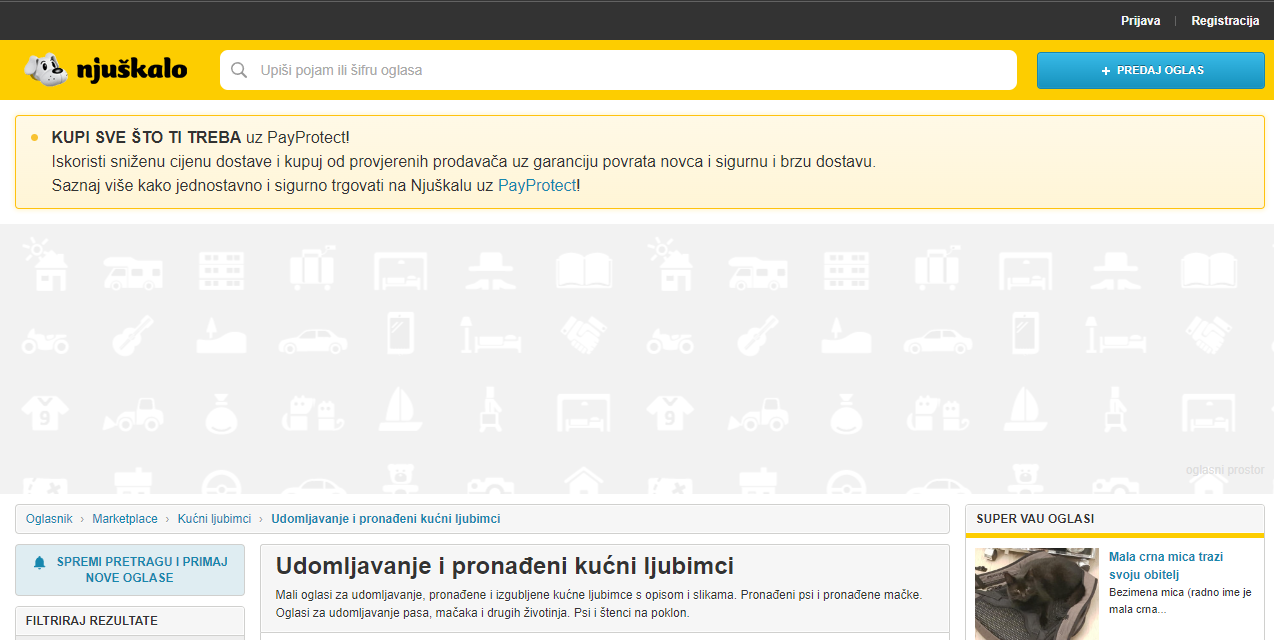
\includegraphics[scale=0.3]{slike/Njuskalo-nestaliLjubimci.PNG}
			\caption{Njuškalo}
			\label{fig:promjene}
		\end{figure}
		
		\textit{Web aplikacija za pronalazak nestalih ljubimaca će predstavljati puno učinkovitije, brže i bolje rješenje u kojem će se korisnici lako i brzo snalaziti. Također, svaki oglas za nestalog ljubimca i komunikacija će biti zasebna cjelina u kojoj se neće preplitati drugi oglasi i po kojima će se lagano i brzo pretraživati dani oglasi. Ovakvu učinkovitost i brzinu ne nude gore navedene web aplikacije poput Facebook-a ili Njuškala.}
		
		\textit{Mogućnost prilagodbe rješenja te moguće nadogradnje projektnog zadatka će svakako biti moguće u budućnosti te će podosta ovisiti o zadovoljstvu korisnika te njihovom mišljenju. Izricanje mogućnosti i potencijalnih rješenja od korisnika se svakako potiče sve s ciljem kako bi web aplikacija predstavljala sve korisnije, učinkovitije i uspješnije rješenje u pomoći i potrazi za korisnikovim nestalim ljubimcem.}
		
		\eject
		
		
		
		\section{Primjeri u \LaTeX u}
		
		\textit{Ovo potpoglavlje izbrisati.}\\

		U nastavku se nalaze različiti primjeri kako koristiti osnovne funkcionalnosti \LaTeX a koje su potrebne za izradu dokumentacije. Za dodatnu pomoć obratiti se asistentu na projektu ili potražiti upute na sljedećim web sjedištima:
		\begin{itemize}
			\item Upute za izradu diplomskog rada u \LaTeX u - \url{https://www.fer.unizg.hr/_download/repository/LaTeX-upute.pdf}
			\item \LaTeX\ projekt - \url{https://www.latex-project.org/help/}
			\item StackExchange za Tex - \url{https://tex.stackexchange.com/}\\
		
		\end{itemize} 	


		
		\noindent \underbar{podcrtani tekst}, \textbf{podebljani tekst}, 	\textit{nagnuti tekst}\\
		\noindent \normalsize primjer \large primjer \Large primjer \LARGE {primjer} \huge {primjer} \Huge primjer \normalsize
				
		\begin{packed_item}
			
			\item  primjer
			\item  primjer
			\item  primjer
			\item[] \begin{packed_enum}
				\item primjer
				\item[] \begin{packed_enum}
					\item[1.a] primjer
					\item[b] primjer
				\end{packed_enum}
				\item primjer
			\end{packed_enum}
			
		\end{packed_item}
		
		\noindent primjer url-a: \url{https://www.fer.unizg.hr/predmet/proinz/projekt}
		
		\noindent posebni znakovi: \# \$ \% \& \{ \} \_ 
		$|$ $<$ $>$ 
		\^{} 
		\~{} 
		$\backslash$ 
		
		
		\begin{longtblr}[
			label=none,
			entry=none
			]{
				width = \textwidth,
				colspec={|X[8,l]|X[8, l]|X[16, l]|}, 
				rowhead = 1,
			} %definicija širine tablice, širine stupaca, poravnanje i broja redaka naslova tablice
			\hline \SetCell[c=3]{c}{\textbf{naslov unutar tablice}}	 \\ \hline[3pt]
			\SetCell{LightGreen}IDKorisnik & INT	&  	Lorem ipsum dolor sit amet, consectetur adipiscing elit, sed do eiusmod  	\\ \hline
			korisnickoIme	& VARCHAR &   	\\ \hline 
			email & VARCHAR &   \\ \hline 
			ime & VARCHAR	&  		\\ \hline 
			\SetCell{LightBlue} primjer	& VARCHAR &   	\\ \hline 
		\end{longtblr}
		

		\begin{longtblr}[
				caption = {Naslov s referencom izvan tablice},
				entry = {Short Caption},
			]{
				width = \textwidth, 
				colspec = {|X[8,l]|X[8,l]|X[16,l]|}, 
				rowhead = 1,
			}
			\hline
			\SetCell{LightGreen}IDKorisnik & INT	&  	Lorem ipsum dolor sit amet, consectetur adipiscing elit, sed do eiusmod  	\\ \hline
			korisnickoIme	& VARCHAR &   	\\ \hline 
			email & VARCHAR &   \\ \hline 
			ime & VARCHAR	&  		\\ \hline 
			\SetCell{LightBlue} primjer	& VARCHAR &   	\\ \hline 
		\end{longtblr}
	


		
		
		%unos slike
		\begin{figure}[H]
			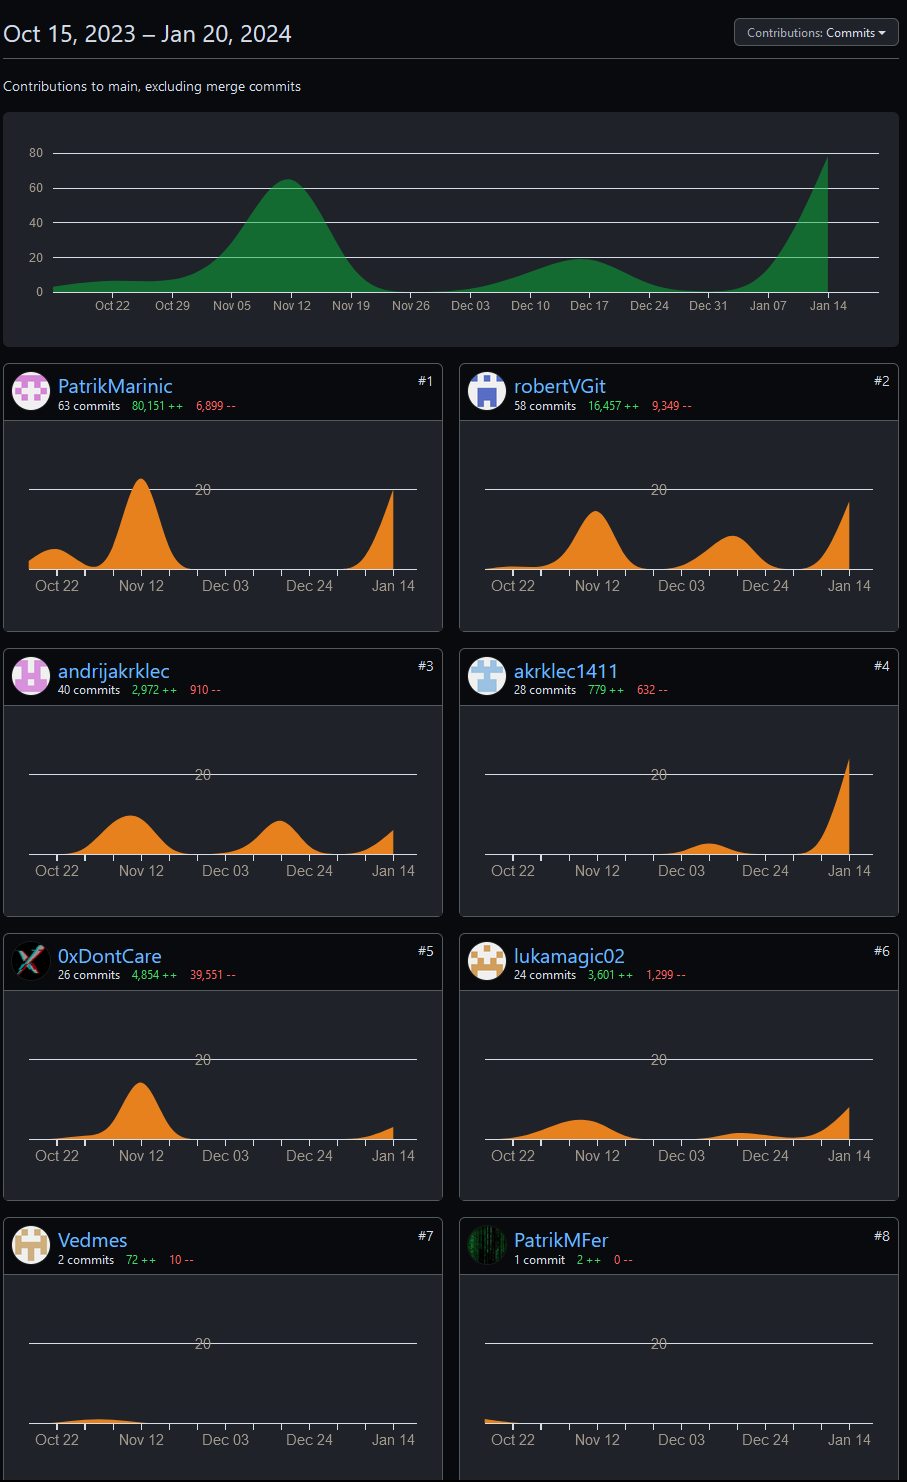
\includegraphics[scale=0.4]{slike/aktivnost.PNG} %veličina slike u odnosu na originalnu datoteku i pozicija slike
			\centering
			\caption{Primjer slike s potpisom}
			\label{fig:promjene}
		\end{figure}
		
		\begin{figure}[H]
			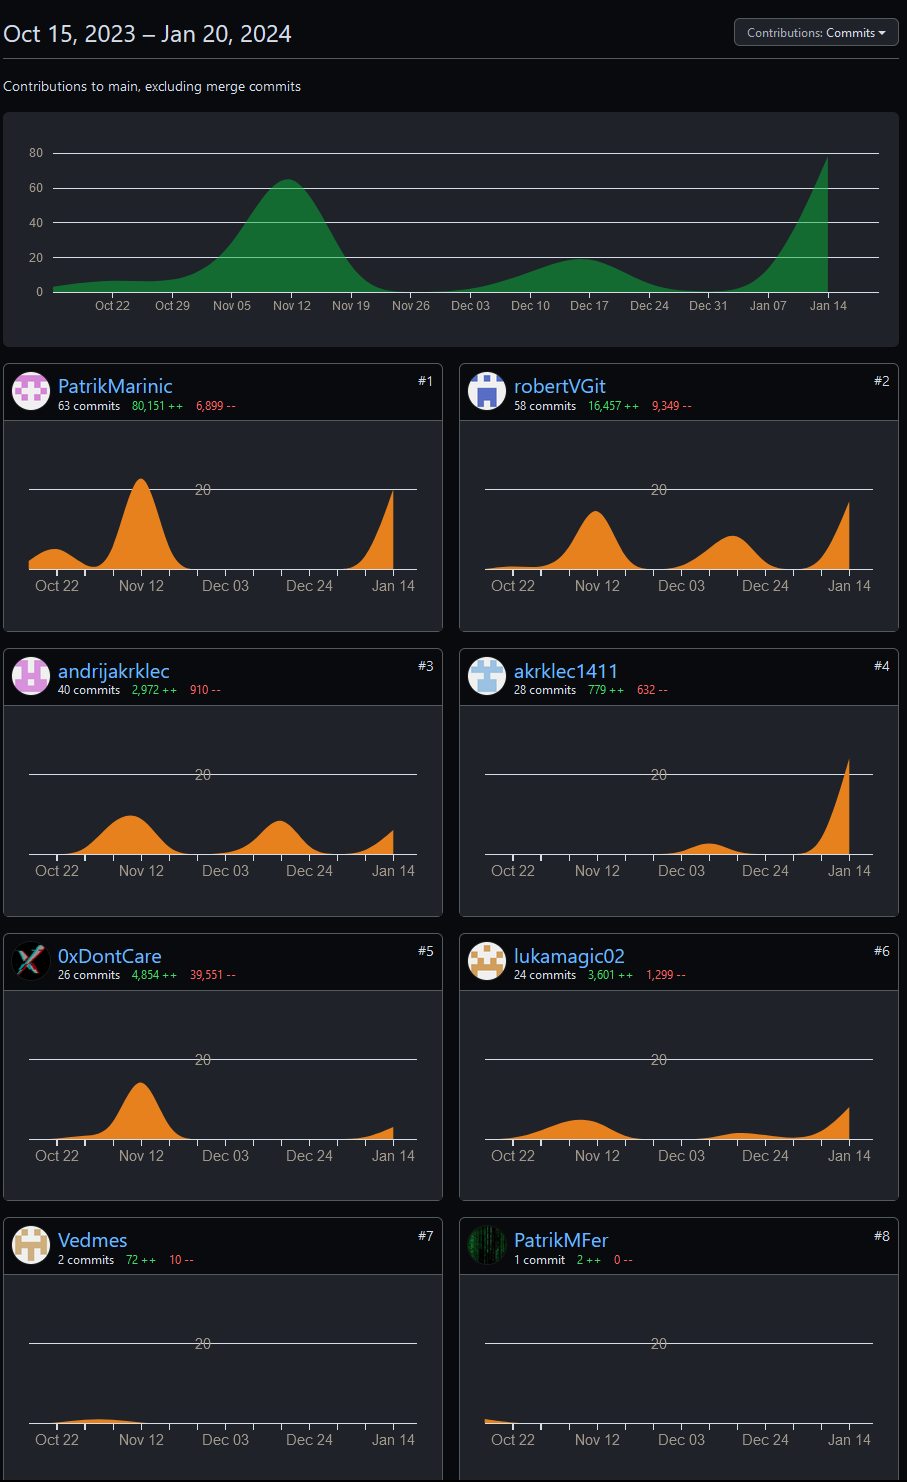
\includegraphics[width=\textwidth]{slike/aktivnost.PNG} %veličina u odnosu na širinu linije
			\caption{Primjer slike s potpisom 2}
			\label{fig:promjene2} %label mora biti drugaciji za svaku sliku
		\end{figure}
		
		Referenciranje slike \ref{fig:promjene2} u tekstu.
		
		\eject
		
	